\begin{infocard}{Proporcionalidad inversa}
    Colocaremos los 3 datos y la incógnita en la tabla igual que los hemos colocado en el caso anterior. Pero aplicaremos una fórmula distinta:
    \begin{figure}[H]
        \centering
        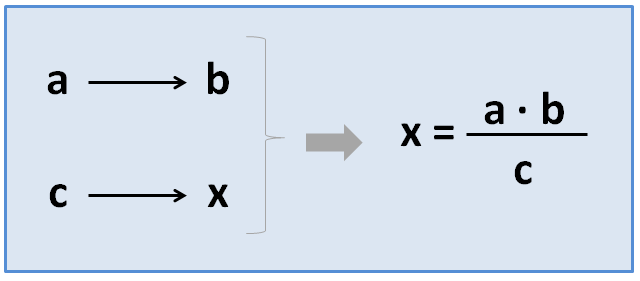
\includegraphics[width=.75\linewidth]{../images/formula-regla-de-3-img3}
        \caption{Solución de una relación proporcional \textbf{inversa} por medio de la regla de 3}
        \label{fig:}
    \end{figure}
\end{infocard}
